\section{Q2. How model checking is performed}
\label{sec:Q2}
%Does the report clearly describe how model checking is being performed? Which parts of the explanation are good? Which parts could be improved and how?

The model checking is performed using the essential state formulae given by figure \ref{fig:stateformulae}.

\begin{figure}[H]
    \centering
    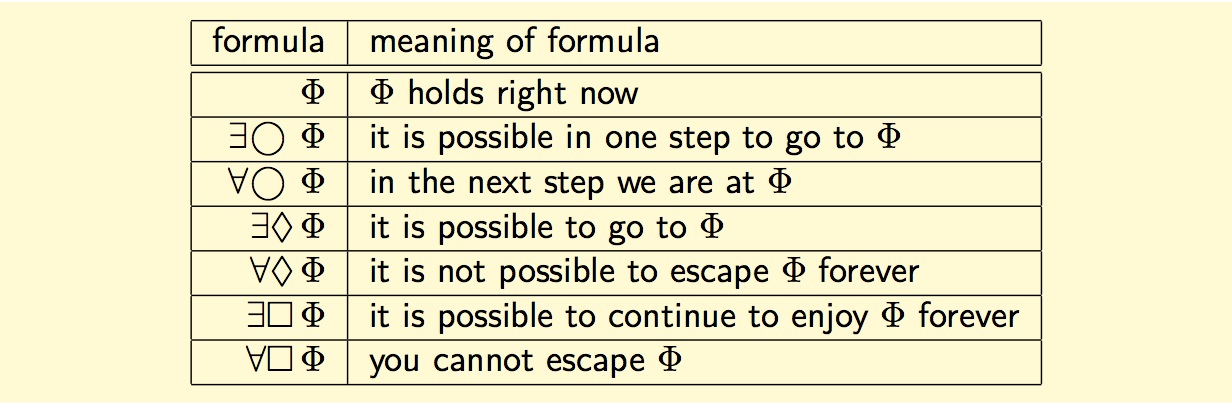
\includegraphics[width=0.7\textwidth]{fig/stateformulae}
    \caption{The given state formulae necessary for model checking}
    \label{fig:stateformulae}
\end{figure}

Furthermore we have implemented $\Phi_1 \wedge \Phi_2$, $\neg \Phi$ and $tt$. \\

The implemented versions of these state formulae are seen in table \ref{tab:implementedformulae}.
\begin{table}[H]
    \centering
    \begin{tabular}{|c|c|}
    \hline
    Symbolic name               & Implemented name \\ \hline
    $tt$                        & \texttt{ctlTT}            \\ \hline
    $\neg \Phi$                 & \texttt{ctlNOT}           \\ \hline
    $\Phi_1 \wedge \Phi_2$      & \texttt{ctlAND}           \\ \hline
    $\exists \bigcirc \; \Phi$     & \texttt{ctlEX}            \\ \hline
    $\forall \bigcirc \; \Phi$     & \texttt{ctlAX}            \\ \hline
    $\exists \lozenge \; \Phi$     & \texttt{ctlEF}            \\ \hline
    $\forall \lozenge \; \Phi$     & \texttt{ctlAF}            \\ \hline
    $\exists \square \; \Phi$      & \texttt{ctlEG}            \\ \hline
    $\forall \square \; \Phi$      & \texttt{ctlAG}            \\ \hline
    \end{tabular}
    \caption{Table of all implemented state formulae with symbolic names and corresponding names of the implemented function/method.}
    \label{tab:implementedformulae}
\end{table}

In order to performing the model checking, the transition system must first be defined as explained in section \ref{sec:Q1}. Once the transition system is defined, the necessary combinations of checks can be performed. Since all the implemented state formulae returns a list of states, any combination of checks are possible. An example of checks is:
\begin{lstlisting}
 ts.checkInitialStates(ts.ctlEX(ts.ctlAG(ts.ctlAP("c"))));
\end{lstlisting}

This example checks if $\varsigma_{\triangleright} \models \exists \bigcirc \forall \square \; c$ (for all initial states). Returning a boolean value.\\

Another example is:

\begin{lstlisting}
 ts.printStates(ts.ctlEX(ts.ctlAG(ts.ctlAP("c"))));
\end{lstlisting}

This example returns (prints in console) the set of states which models $\models \exists \bigcirc \forall \square \; c$. \\

As seen, the state formulae are implemented as functions/methods allowing one to choose which tests to run in the model checking. The functions/methods are explained in more detail in the following section.